\section{Introduction}

\begin{frame}
	\frametitle{Problem}
	
	\vspace{0.3cm}
	
	\begin{center}
		\begin{tikzpicture}
			\node at (0,0) [draw=black,ultra thick,inner sep=0pt]
			{
				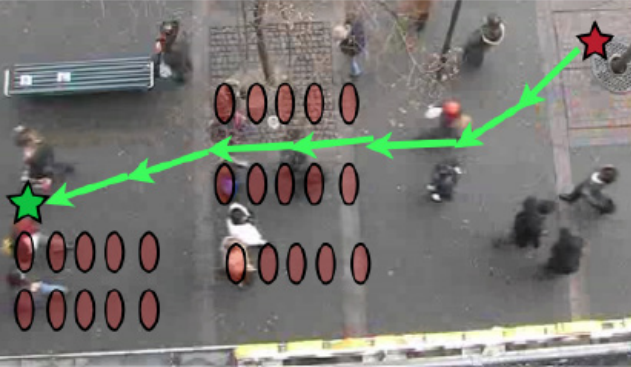
\includegraphics[scale=0.45]{Figures/Problem.png}
			};
		\end{tikzpicture}
	\end{center}
\end{frame}

\begin{frame}
	\frametitle{Motivation}
	
	\vspace{0.4cm}
	
	\Large
	
	\begin{block}{Objective}
		\textbf{Making} a robot to \textbf{function autonomously} in dynamic environments
		wherein other decision making agents, such as people or other robots, are present
	\end{block}
	
	\vspace{0.3cm}
	
	Example of application fields:
	
	\begin{itemize}
		\item Automatic video surveillance
		\item Human-Robot Interaction
		\item Domestic robots
	\end{itemize}
\end{frame}
